\documentclass[10pt]{article}
\usepackage[margin=0.85in]{geometry}
\usepackage[T1]{fontenc}
\usepackage{amsmath,amssymb,booktabs,longtable,hyperref,tikz}
\usetikzlibrary{arrows.meta,positioning}
\hypersetup{colorlinks=true,urlcolor=blue}
\title{\textbf{Four-Lane Fractal Holonet}\\Exact W33 Edge-Coloring, Three-Slot Switching, and Optical Interface Budget}
\author{W33-Theory hardware programme}
\date{23 October 2026}
\begin{document}\maketitle
\begin{abstract}
This addendum converts the four-line-gateway proposal in the main fractal Holonet blueprint into a verified, bandwidth-accounted network. A twelve-perfect-matching certificate of the symplectic point graph $W(3,3)$ programs four line-address gateway lanes over three collision-free slots. The resulting sparse parent needs 240 inter-child logical links rather than 960; its 1,600-node level-two recursive graph has exact diameter seven (versus five in the fully replicated design). This is a logical graph/scheduler result, not a physical optical implementation, measured latency, or demonstration of quantum computation.
\end{abstract}
\tableofcontents
\section{Source stack and corrected graph semantics}
Primary sources: \texttt{holonet\_machine\_blueprint.pdf} (268 pages),
\texttt{photonic\_holonet.pdf} (351 pages),
\texttt{holonet\_practical\_implications.pdf} (23 pages), and
\texttt{papers/forty\_points/main.pdf} (203 pages in the audited snapshot).
The existing \texttt{papers/fractal\_holonet\_architecture\_20261023.tex}
defines two baseline graph choices. Its 40-child recursion is consistent
with BT827; it is not the withdrawn ternary recursive RTL interpretation
from Pass 2686. Neither BT827's eight chart moves per digit nor
Holotrade's higher-level routing heuristic is automatically a
distance bound on the newly defined sparse optical-link graph.

\section{A frozen perfect-matching proof certificate}
Represent W33 points by normalized projective vectors in $\mathbb F_3^4$.
The alternating symplectic pairing is
\[
\langle u,v\rangle =u_0v_1-u_1v_0+u_2v_3-u_3v_2\pmod 3.
\]
For distinct $u,v$, adjacency is equivalent to zero pairing.
The graph is $\operatorname{SRG}(40,12,2,4)$, with 240 undirected edges.
The code freezes a partition
\[
E(W33)=M_0\sqcup M_1\sqcup\cdots\sqcup M_{11},
\quad |M_k|=20,
\]
where each $M_k$ is a perfect matching. Unlike a citation to a
non-reproducible search, the 12 lists are committed as integers
$e=40u+v$ with $u<v$, and verified against an \emph{independently
generated} exact adjacency relation. Every group covers each of the
40 vertices once; all 240 edges occur in exactly one group.

The selected isotropic gateway line is
\[
L=(0,31,32,33).
\]
All off-line vertices have exactly one neighbor on $L$.
For edge $(u,v)\in M_k$, set
\[
\operatorname{lane}(u,v)=k\bmod4,\quad
\operatorname{slot}(u,v)=\lfloor k/4\rfloor,\quad
\operatorname{gateway}(u,v)=L_{k\bmod4}.
\]
Every child has three assigned neighbors on each of its four lanes.
There is no double-use of a lane at a child within one slot.

\section{Connection, switching, and timing diagrams}
\begin{center}
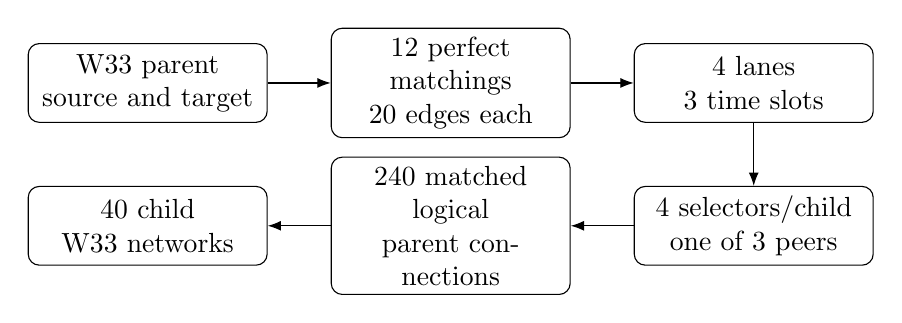
\begin{tikzpicture}[>=Latex,blk/.style={draw,rounded corners,align=center,text width=28mm,minimum height=10mm},node distance=8mm]
\node[blk](route){W33 parent\\source and target};
\node[blk,right=of route](match){12 perfect matchings\\20 edges each};
\node[blk,right=of match](slot){4 lanes\\3 time slots};
\node[blk,below=of slot](switch){4 selectors/child\\one of 3 peers};
\node[blk,left=of switch](links){240 matched logical\\parent connections};
\node[blk,left=of links](end){40 child\\W33 networks};
\draw[->](route)--(match);\draw[->](match)--(slot);\draw[->](slot)--(switch);
\draw[->](switch)--(links);\draw[->](links)--(end);
\end{tikzpicture}
\end{center}
At each slot, four matchings yield $4\cdot20=80$ active
inter-child edge transfers, occupying the 160 lane-specific
endpoints. Over three slots, all 240 neighbor pairs receive
one scheduled transmission opportunity.
This is \emph{optimal} for the stated single-transfer-per-lane
contract because $12/4=3$ slots are necessary. Optical propagation
time, control electronics, feedforward, time-bin guard intervals,
bidirectionality and traffic queueing are unspecified.
A plausible optical implementation would require four 1-to-3
switch selectors per child. A naive binary tree uses two 2-by-2
switch elements per selector, giving $40\cdot4\cdot2=320$ nominal
elements per parent before loss, phase trim, monitors and layout;
this is an \emph{architectural estimate}, not a PDK-verified bill
of materials.

\section{Scaling comparison and route limitation}
With $40^n$ leaves, define $B_n=(40^{n-1}-1)/39$
higher-level 40-child parents. The three choices have undirected
logical link counts:
\[
\begin{aligned}
E_{\mathrm{cart}}(n)&=240n40^{n-1},\\
E_{\mathrm{4gateway}}(n)&=240\cdot40^{n-1}+960 B_n,\\
E_{\mathrm{sparse}}(n)&=240\cdot40^{n-1}+240 B_n.
\end{aligned}
\]
\begin{center}
\begin{tabular}{rrrr}
\toprule
Depth & Cartesian links & Four-gateway links & Sparse links\\
\midrule
1 & 240 & 240 & 240\\
2 & 19,200 & 10,560 & 9,840\\
3 & 1,152,000 & 423,360 & 393,840\\
\bottomrule
\end{tabular}
\end{center}
At level two, all-source BFS gives exact graph diameters
four, five, and seven, respectively.
The sparse gateway route resolves the first differing parent
digit through at most two W33 hops, moves the suffix to the
edge's assigned gateway lane, crosses, and recursively
restores the destination suffix. Its \emph{constructive} bound is
\[
D_1=2,\qquad D_n\le 2D_{n-1}+3,\qquad
D_n\le5\cdot2^{n-1}-3.
\]
This is conservative and exponential in recursion depth;
the claimed $O(n)$ chart-routing bound in other documents
is not yet transferred to this \emph{different sparse graph}.
Finding a better route or topology while keeping a bounded
physical link budget is a central follow-up.

\section{Optical fabrication and falsification contract}
The prior 16-mode Halmos/MZI compiler is a distinct optical
transformation. It is \emph{not} a 40-child switch network merely
because both architectures have optical components.
The following independent physical claims remain open:
\begin{longtable}{p{0.28\linewidth}p{0.58\linewidth}}
\toprule Requirement & Evidence needed\\\midrule
Physical PDK switch & 1-to-3 cell S-parameter/transfer model,
electrode routing, allowed waveguide layers and geometry\\
Chip-level connectivity & 240 link instances per parent,
optical LVS, bend/crossing losses, DRC and post-layout extraction\\
Real timing & Controller-to-actuator delay, switch-settling
time, path propagation, time-bin guard and clock synchronization\\
Control contention & Concurrent demands, arbitration,
buffer requirements, starvation and backpressure model\\
Quantum validation & Source and detector efficiency,
photon indistinguishability, noise, conditional quantum output states\\
Scaling & Packaging, source power, physical density,
fiber/interposer network cost and measured path loss\\\bottomrule
\end{longtable}
A graph-theoretic three-slot schedule is not a statement that
three optical clock cycles suffice, nor that all 240 links can
operate simultaneously. Reports of a fabricated device,
universal quantum computer, or experimentally demonstrated
fractal scaling would be unsupported.

\section{Executable replication}
Run:
\begin{verbatim}
python analysis/w33_fractal_port_fabric_20261023.py --depth 3 --exact-level2
python analysis/w33_fractal_four_lane_scheduler_20261023.py --depth 3 --exact-level2
python -m pytest -q tests/test_w33_fractal_port_fabric_20261023.py
python -m pytest -q tests/test_w33_fractal_four_lane_scheduler_20261023.py
\end{verbatim}
Machine-readable manifests:
\texttt{data/w33\_fractal\_port\_fabric\_20261023.json} and
\texttt{data/w33\_fractal\_four\_lane\_schedule\_20261023.json}.
The test run on 23 October 2026 passed 15 regressions across both
modules and independently exhaustively checked the level-two
sparse diameter, without asserting a foundry or physical
optical switch implementation.
\end{document}
